
%proofread!

\documentclass[draft,jgrga]{agutex}
\usepackage[dvips]{graphicx}
\usepackage{amsmath}
\usepackage{multirow}

\usepackage{tabularx}
%\usepackage{lineno}
%\linenumbers*[1]

%\noindent $>$latex file \\
%\noindent $>$dvips -P pdf -o file.ps file.dvi \\
%\noindent $>$ps2pdf13 file.ps file.pdf

\authorrunninghead{GUTOWSKI ET AL.}
\titlerunninghead{Radar uncertainty}

\authoraddr{D. Blankenship, Institute for Geophysics, University of Texas at Austin}
\authoraddr{Gail Gutowski, Department of Geosceinces, University of Texas at Austin (gail.gutowski@utexas.edu)}
\authoraddr{Charles S. Jackson, Institute for Geophysics, University of Texas at Austin}
\authoraddr{Duncan Young,  Institute for Geophysics, University of Texas at Austin}


\begin{document}

\title{Uncertainty of ice-penetrating radar and corresponding uncertainty at Byrd Ice Core, Antartica}

\authors{Gail. Gutowski, \altaffilmark{1,2}} Charles S. Jackson, \altaffilmark{2} D. Young, \altaffilmark{2} D. Blankenship, \altaffilmark{2} 

\altaffiltext{1}{Department of Geosciences, University of Texas at Austin, Austin, TX, USA}
\altaffiltext{2}{Institute for Geophysics, University of Texas at Austin, Austin, TX, USA}



\begin{abstract}
%Data from radar-sounding surveys of West Antarctica are used to determine the age of observed radar horizons near the Byrd ice core, Antarctica~\citep{gow1968}. We emphasize inclusion of uncertainty in radar- and ice-related sources of uncertainty. The analysis is based on a basic ice-flow model developed by~\citet{schwander2001}. The model assumes no basal melting, zero velocity at the bed, and linear strain rate below 1200 meters depth.

%A Bayesian uncertainty analysis is performed to reduce uncertainties and make the best use of the available data. The analysis quantifies observational limitations of the analysis, informing future uncertainty reduction through refinement of observational techniques. A Research Plan outlines a Bayesian approach to develop a new chronology of the Byrd ice core which takes into account theoretical and measurement uncertainties in depth and age of prominent layers observed in the ice column. The method employs Markov Chain Monte Carlo modeling to invert for accumulation and strain as functions of depth.


%Our goal is to determine the uncertainty in age and depth of observed radar reflection horizons near Byrd Station, West Antarctica through comparison with the Byrd ice core record. Here we show the distribution of age and depth with their modeled uncertainties based on the methods described above.  

%We determine the uncertainty in comparing age-depth relationships from ice core records to 




Ice-penetrating radar (IPR) is a useful tool for investigating past and present climatic conditions and developing a better understanding of ice dynamics.  Interpretation of the data for the purpose of  climate or ice dynamics studies requires accurate dating of internal radar reflection horizons. This can be achieved through the combination of IPR and age-depth profiles established from ice cores. To do so, it is therefore necessary to consider contributions to uncertainty from both aircraft-based IPR data and ice-core dating techniques. The Airborne Geophysical Survey of the Amundsen Sea Embayment (AGASEA) project has provided a wealth of focused IPR data for West Antarctica. We consider uncertainty due to phase selection and bandwidth in 10 bright radar horizons observed near Byrd Station, West Antarctica to determine the depth range from which each of the horizons originates. We use a simplified ice flow model to transfer an age-depth relationship for the Byrd ice core to the radar horizons using a Bayesian inversion method. The inversion considers uncertainty in the ice core dates to determine model parameters. A new ensemble of age-depth profiles for Byrd Station is then obtained through forward modeling of the inverted model parameters.






 but interpretation and analysis of the data requires an understanding of the uncertainty introduced by aircraft-based IPR. 

ADD: \\
%       where did accum come from?\\
%	comparison to Morley flow?
%	discussion of layers/age deeper in the ice sheet
	add more numbers/tables;\\
	fill out who? references;\\
%	add plenty of references\
%	add bibtex references
%	further description of schwander model?;\\
%	future work
%	discussion of correlation between layers
%	discussion of wa-wa
%	discussion of ECM?
%	where did sd's on age come from? -- NOT 3percent!;\\
%	proofread\\
	fix figures \\


\end{abstract}

\begin{article}
\section{Introduction}

The West Antarctic Ice Sheet (WAIS) has become an important focus of glaciological research because it is the last marine ice sheet on Earth. A full 75$\%$ of the ice sheet is based below sea level, leaving the region susceptible to the Marine Ice Sheet Instability Problem \citep{joughin&alley2011}. The problem describes the potential instability of WAIS in the event of grounding line retreat. This process acts as a positive feedback to the system, resulting in accelerated retreat of the grounding line until the ice sheet reaches a steady state position upstream. Marine ice sheet instability could therefore be responsible for a rapid disintegration of up to 75$\%$ of the West Antarctic ice sheet. This scenario would result in a global sea level rise approaching 5m \citep{joughin&alley2011}, threatening tens of millions of individuals worldwide \citep{mcgranahan2007}. It is therefore important to gain a better understanding of ice flow in West Antarctica in order to gauge its susceptibility to catastrophic mass loss in response to climate change.  

Ice-penetrating radar surveys of ice sheets provide a glimpse into the interior of the ice sheet, where other observational methods provide little information. Reflection horizons in the radar reveal internal horizontal layering in the ice sheet which can be interpreted at isochronous layers of ice \citet{eisen2004}.  These layers provide one avenue for developing an understanding of ice dynamics.  Each year, snow accumulates on the surface of the ice sheet. The physical properties of this snow contain information about climatic conditions at the time of deposition. For instance, the oxygen isotope$\delta^{18}O$ can be used as a proxy for temperature. Over time, the surface layer is covered with the accumulation of subsequent years and becomes buried in the ice column. This process produces isochronous layering within the ice seet which contains information about surface conditions at the time of accumulation of that layer. This makes it possible to recreate ancient climates from long-buried layers of ice.
 
%For example, the thickness of an isochronous layer which corresponds to the accumulation over the period of deposition of that layer. As the layer is advecting down into the ice sheet, it will thin as a result of gravitational compaction, but it is possible to correct for this effect and so retain some information about accumulation rate. Accumulation rates and patterns of accumulation are related to several climatic factors of interest including air temperature and atmospheric CO$_2$ concentration ~\citep{neftel1988,alley2000}. 

Radar horizons can be tracked over large glaciated regions, in some cases tracing ice flow across hundreds of kilometers, as in the case of West Antarctica ~(\citet[e.g.]{holt2006}). As mentioned earlier, this allows for studies of paleoclimate over large regions of an ice sheet. In East Antarctica, tracking internal layers using ice-penetrating radar presents the opportunity to directly compare ice core analyses between stations located throughout the region. This cross-correlation provides an unprecedented opportunity for constraining the uncertainty of ice core chronologies. 

Some of the latest technology in aerogeophysical surveys of Earth’s major ice sheets includes focused synthetic aperture radar (SAR) techniques. Focused radar products provide an even better picture of glacial isochrones by including additional clutter reduction and preserving echoes from sloped layers. This enhances our ability to detect and track layers, in increasingly more complex englacial environments \citep{peters2005}.

It is possible to learn about ice flow from drawdown and deformation observed in the layers. Layer draw down, in which layers move deeper in the glacier (with or without a corresponding change in bed topography) may be indicative of basal melting. In some cases, for example, observations reveal layers disappearing, a sign that ice is (or was) melting. This could correspond to areas of fast-moving ice (past or present) such as an ice stream, or may indicate an area of increased geothermal heating. 

Because internal layering encodes information about accumulation rates and ice deformation, it can be used to develop a picture of ice dynamics. One of the main obstacles in ice sheet modeling is the uncertainty surrounding basal boundary conditions. One way to explore this problem is to use surface observations to invert for basal parameters \citep{thorsteinsson2003}. Dynamical information about the flow of ice within the column, derived from analyses of internal isochrones can further inform these inversion problems to more accurately describe and reduce uncertainties in basal boundary conditions. In order to accomplish this, it is necessary to assign ages to internal layers observed with radar by comparison to age-depth profiles obtained from ice cores. The accuracy of dating intenral radar horizons therefore depends on the uncertainty in the radar observations themselves and the uncertainty in ice-core dating. \cite{eisen2004} evaluated this uncertainty for ground-based radar in the top 100 m of the East Antarctic Ice Sheet. We approach the problem using aircraft-based observations of WAIS and consider radar horizons in the top 1300 m of the ice sheet.   


\section{Data}

Radar-echo sounding data was obtained in December 2004 as part of the Airborne Geophysical Survey of the Amundsen Sea Embayment (AGASEA) project \citep{holt2006}. The radar line passed 870 m from the Byrd ice core site. The plane was travelling at 67 m/s at an elevation of 550 m above the ice. The data includes two-way travel times (the time it takes for a radar pulse to be transmitted, reflect off a layer, and return to the receiver) in microseconds. The data were collected with a 15 MHz bandwidth. We use ten strong radar horizons that were hand picked using the seismic imaging software \textit{GeoFrame}.

A volcanic chronology was used to quantitatively compare our calculated age-depth relationship to the age of layers in the Byrd ice core \citep{hammer1994} for comparison to our model. The chronology was developed using the electrical conductivity method. The chronology includes dated volcanic events that cover an age range from 709 BP to more than 18,000 BP. These events correspond to a depth range from 97.8 m to 1890 m below the 1968 surface of the Byrd ice core \citep{gow1968}.

Ice density data as a function of depth were obtained from the original analysis of the ice core \citep{gow1968}. The data were used to account for the varying density of ice in the upper part of the ice sheet. The result was used to apply a firn correction constant to the ice thickness at Byrd ice core. 





\section{Sources of Uncertainty}\label{unc}
There are many sources of uncertainty inherent to the way in which
data is collected, analyzed, and understood. We have included the
following sources of uncertainty.

\subsection{Uncertainty in radar two-way travel time (TWTT)}

Radar horizons, surfaces of constant TWTT, are hand-picked using seismic interpretation software. This allows a user to select strong reflectors from a radargram and trace them along a radar line. However, there is a limit to the accuracy of tracking a single phase of a radar reflection. The accuracy depends on the resolution of the sampling rate of the radar transmitter as well as considerations of noise. For high sampling rates, the uncertainty in phase selection is typically $\frac{\lambda}{4}$, but can be as accurate as $\frac{\lambda}{2}$ for data with high signal-to-noise where $\lambda$ is the wavelength of the electromagnetic pulse.  The sampling rate for the data used here varies from 5 ns to 20 ns. To be conservative, we assume a 10 ns resolution when tracking the phase of reflections from the surface of the ice sheet and from each internal layer. We treat the surface and internal layers separately in this instance. 

To convert TWTT uncertainty into units of depth, we scale the time by the velocity of electromagnetic wave propagation in the medium. The pulse travelled from the aircraft to the ice sheet surface with velocity, c, the speed of light, and then slowed to the velocity of electromagnetic wave propagation in ice, which we take to be $\textit{c}_i$ = 1.69 x 10$^8$ m/s before reaching the internal layers and reflecting back. The corresponding 1$\sigma$ uncertainty is $\sigma_{surf}$ $\sim$0.3 m for the surface reflector and $\sigma_{lay}~\sim~$0.17 m for each of the internal layers, assuming the uncertainty is gaussian.
 
The uncertainty associated with picking the elevation of the surface is considered a systematic error because the same surface elevation will be used to normalize all of the internal layers. The TWTT uncertainty of each of the internal layers is applied randomly because each of the individual layers need not have the same uncertainty. This is because the reflection from each layer need not have the same phase with respect to the sampling rate. To account for this, we assume the TWTT to be normally distributed and sample randomly from this distribution for each of the internal layers independently.

The finite bandwidth of the data means that even an infinitesimally thin layer of ice will appear in the survey to have a finite width. Our data uses a pulse bandwidth of 15 MHz. This translates to a 1$\sigma$ depth uncertainty of 5.63 m, obtained from considering both the bandwidth frequency and the velocity of electromagnetic radiation in ice. This uncertainty is applied as a random, normally-distributed error in the depth of each of our selected layers. 




\subsection{Uncertainty in determination of age}\label{ageunc}

%Each year fresh snow accumulates on the top of the ice sheet,
%burying the previous season's snowfall. As layers of ice descend into
%the ice sheet, the layers become thinner, as air from the surface is
%squeezed out and gravity compacts the ice. This thinning makes it
%increasingly difficult to distinguish one layer from another at
%depth while in shallow regions, it maybe be possible to simply count
%layers by eye and therefore determine the age of those layers. 

%The uncertainty associated with determining ages for ice layers is a
%function of depth;
%-delta age \\
%-landmarks like 10Be, CH4, F \\
%-ecm method accuracy \\
%-correlation with bc89? \\


Each year, fresh snow accumulates on top of the ice sheet, burying the previous season’s snowfall. As layers of ice descend into the ice sheet, they become thinner because air is squeezed out and gravity compacts the ice. This thinning makes it increasingly difficult to distinguish one layer from another at depth. In shallow regions, it is possible to count layers by eye to determine the age of near-surface isochrones; however, this is harder to do deep in the ice sheet.

The uncertainty associated with determining ages for ice layers is therefore a function of depth. Several sources are responsible for increased uncertainty with depth. There are two methods of dating ice cores: by “ice” age or by “gas” age \citep{bender2006}. This has to do with the fact that ice in the upper part of the glacier still contains atmospheric gases until such a depth as pore closure occurs, squeezing out the air. Because the air is able to penetrate below the surface and into the firn layer, ice at a given depth tends to be older than the air at that depth. This discrepancy leads to an ambiguity in the true age of the ice if atmospheric chemistry is used to determine the age of the ice. The uncertainty has been well-established using the GRIP ice core \citep{blunier1998}, which we use in the upper part of the ice sheet and take to be $\sigma_{age} = \pm$ 10 a.

Isotopic dating is common among ice core chronologies. Landmark events for concentrations of Beryllium-10, methane, and fluorine (to name a few) are matched to chemical analyses of the ice \citep[e.g.]{schwander2001}. Accepted dates for these events are then mapped onto the ice core. However, there is uncertainty in when these events occurred which needs to be accounted for in the ice core chronology.

--> Isotopic events -- which did I use? when did they happen? what's uncertainty? list numbers.

The Electrical Conductivity Method (ECM) is another approach to dating ice. It involves measuring the conductivity of ice at different depths \citep{hammer1994}. This conductivity is associated with the composition of the ice, characterized by its acidity level. Layers of ash embedded in the ice, for example, will have a distinct conductivity. These ash layers are then attributed to known (or assumed) volcanic events. The ECM method is particularly useful in deep parts of the ice column where it is difficult to otherwise distinguish isochronous layers due to layer thinning. For the deep part of the ice sheet we therefore assume an uncertainty calculated from the ECM method. For layers older than X a, we assuming $\sigma_{age}$ = X a. Note that we include this uncertainty for completeness in our model, but the 10 layers evaluated in this study are believed to be less than 20,000 a old.

Table~\ref{blah} summarizes the uncertainty we assign to observed ages as a function of depth.





\section{Method}\label{method}

We use an ice flow model adapted from \citet{morland2009} to determine the age of internal layers near the Byrd ice core drilling site in Antarctica.  The simple flow model has the following form:
\begin{equation}
\frac{\overline{z}}{h_0} = \frac{1}{1-r} [1 - exp(-s \overline{t}]
\overline{z} = h_0 - z
r = \frac{b}{q}
s = s_ds_0
\end{equation}

where depth, $\overline{z}$ is defined to be 0 at the base, $h_0 =$ 2164 m is the depth at the ice sheet surface, b is basal melting rate, q is the accumulation rate, and $\overline{t}$ is the age corresponding to $\overline{z}$. The optimum constant strain rate, $\textit{s}$, is used to achieve reasonable correlations between the model and observations; $s_0$ is the initial strain rate and $s_d=$0.722 for the Byrd ice core. The model assumes isostatic equilibrium, constant ice density, uniform strain rate in $\textit{z}$, and r $<$ 1 (i.e. nonnegative mass balance in the ice column). Note that it is difficult to know accumulation rate on its own due to layer thinning within the ice column. As such, we consider layer thickness instead of layer accumulation because it can be physically measured using the techniques described previously. Further, while depth in the model, $\overline{z}$, is defined so that $\overline{z}$(base) $=$ 0, the following analysis is discussed in terms of depth $\textit{z}$, where $\textit{z(surface)} = 0$.

We use the flow model to invert for layer thickness as a function of depth, $\textit{q}$ and strain scale factor, $\textit{s}$ using an observed age-depth relationship and then use the resulting parameters to evaluate the age of 10 prominent radar horizons. First, we use a Markov Chain Monte Carlo technique known as the Metropolis algorithm to invert for layer thickness and strain scale factor. We use a stepwise function to describe layer thickness, breaking it into four depth regimes:

$\textit{z} = $
%\begin{cases}
%\textit{z_1}, \text{ m} \\
%\text{\textit{z_2}, \ge 150 m and $<$ 1024 m} \\
%\text{\textit{z_3}, \ge 1024 m and $<$ 1294 m} \\
%\text{\textit{z_4}, \ge 1292 m}
%\end{cases}

These regimes were chosen based on a function of layer thickness developed by \citet{who?} in which shifts in layer thickness are seen at the above transition points.

The Metropolis algorithm utilizes prior knowledge about the model parameters (accumulation and strain scale factor) to step through parameter space. We use truncated uniform priors on our parameters, allowing them to take on values within a reasonable range. We allow accumulation to vary between 0 cm/a and 30 cm/a while the strain scale factor may take values between 0 and 1.7.  The model is intialized using random parameter values within these ranges.

At each step, we evaluate the age model at every point in the ice column based on the parameters.  An associated cost is calculated  as a measure of the fit of that instance of the model to observations. The cost is described by equation~\ref{cost}:

\begin{equation}\label{cost}
cost = e^\frac{(Age_{model}~ - ~Age_{obs})^2}{(\sigma_{obs})^2}
\end{equation}

where $Age_{model}$ is evalation of the \citet{morland2009} ice flow model for a given accumulation and strain scale factor. $Age_{obs}$ and $\sigma_{obs}$ come from the volcanic age-depth function and we allow for the aforementioned uncertainty in $Age_{obs}$ (see Table~\ref{age_unc})to loosen the constraint on the cost function. At each iteration the algorithm makes a decision about whether or not to accept the combination of parameters based on the cost: if the cost of the $\textit{n}$th iteration is less than the cost of the $\textit{(n-1)}$th iteration, the set of parameters is accepted. This means that the $\textit{n}$th set of parameters is a better fit to the data (because the cost has decreased). If the cost of the current nth iteration is greater than the cost of the $\textit{(n-1)}$th iteration, the set of parameters is accepted with probability $exp[-\frac{cost_n~-~cost_{n-1}}{2}]$, the Metropolis probability. The algorithm then does a random walk through parameter space, comparing the cost of each step to the step before.

The Metropolis algorithm uses the principles of Bayesian statistics to generate a large number of distributions that could describe the probability of an outcome. In our case, the outcome is that a radar horizon at a given depth takes on a particular age based on knowledge about ice flow. We generate 20,000 sets of parameters (accumulation and strain rate) that characterize  physically reasonable of ages for each horizon depth. Age uncertainty, in terms of a variance, can be extracted from this distribution of ages.With a distribution of ages for every depth in the ice column, we then create depth probability distributions (one for each age distribution we calculated previously) for each of the 10 layers. We assume that all uncertainties can be represented as gaussian. 

To find the sampling rate uncertainties, we draw a single value from the probability distribution for the surface reflector, described by $\sigma_{surf}$. We then randomly sample ten values from a probability distribution described by $\sigma_{lay}$, resulting in a radar sampling rate for each of the layers. The bandwidth uncertainty is found in the same fashion as the sampling rate error for the layers. The bandwidth and sampling rate uncertainty vectors are summed.  We also add a correction for firn density and account for additional accumulation between 1968 (when the core was drilled) and 2004 (when the radar line was flown) assuming a constant accumulation rate of 11 cm/a.The result of this process is a single probability distribution for each layer, describing the depth uncertainty for that layer. We then use the forward model of ice flow to find ages (sampled from the previously calculated distribution) that correspond to the range of possible depths of each layer. This gives a range of ages for each layer. The final result is an ensemble of age-depth profiles which each describesthe ten prominent radar horizons and take into account uncertainties in both age and depth.






\section{Results}




Figure~\ref{depthhist} shows the distribution of modeled depths associated with each ice layer of interest from radar observations near Byrd Station, West Antarctica. The spread in the distribution is indicative of uncertainty due to observational methods. Table~$\ref{results}$ shows the standard deviation of depth for each of the 10 chosen layers, assuming the errors to be guassian. See Section~$\ref{ageunc}$ for a full discussion of the sources of uncertainty included in this analysis. The uncertainty in each layer depth is more or less constant with depth. However, deeper in the ice sheet, near X m and Xm,  multiple radar horizons observed as being distinct are consistent within uncertainty with being from the same source. 

The corresponding age distributions are shown in Figure~\ref{agehist} and again assume gaussian errors. Table~\ref{results} shows the mean and standard deviation for each peak. Due to increased uncertainty in ice core dating, age uncertainty increases with depth. As with depth, layers at X m and X m are consistent with originating during the same period. This ambiguity makes it clear that robust uncertainty quantification is critical for the interpretation of internal layers; dynamic analyses require that radar horizons be distinguished in order to obtain a time-dependent profile of ice flow. 

Figure~$\ref{spaghetti}$ shows an ensemble of modeled age-depth distributions for the 10 picked radar layers. The distributions are trained on the observed volcanic record at Byrd Station, allowing for uncertainties in both depth and age. Note that both systematic and random sources of uncertainty are included. Crossing lines indicate that random uncertainty plays a significant part in the age-depth distribution of ice layers at Byrd Station. Spread between ensembles that do not cross is representative of systematic uncertainties in the model. 

As described in Section~$\ref{method}$, the model is based on five parameters: layer thickness parameters in four depth regimes and a ratio of surface to bed ice velocity. Figure~$\ref{accum}$ shows the distributions of the layer thickness parameters, which are used as a proxy for accumulation in the model. As expected due to layer thinning with depth, mean layer thickness decreases with depth. The modeled layer thickness is consistent with layer thickness at the Western Divide determined by \citep{neumann2008} abov 1294 m; Table~\ref{accums} shows a comparison between the two. We expect layer thickness to be at a maximum at the divide and therefore reasonable values at Byrd Station should be less than those at the divide. Our modeled layer thickness below 1294 m is larger than shallower modeled thicknesses and greatly exceeds the layer thickness at the divide at this depth. However, this depth corresponds to only the deepest radar horizon of interest, so it should not affect the result.

\section{Discussion and Conclusion}
Uncertainty associated with two-way travel time in airborne ice-penetrating radar surveys of Antarctica is not thoroughly understood. We seek to quantify that uncertainty and its affect on depth and age uncertainties near Byrd Station, West Antarctica. These results will provide an fundamental contribution to the interpretation of ice-penetrating radar observations. Extending the analysis to determine an ensemble of new age-depth distributions near Byrd ice core provides information about dynamic layer deformation in the region. Improved understanding of layer deformation in the Thwaites Glacier catchment, where Byrd Station resides, will contribute to improved ice flow models of the region and a more complete picture of the dynamic history of West Antarctica which will ultimately improve projections of future sea-level rise. 

Our approach employs a simple ice flow model and basic parameter assumptions which we will improve upon in the future. The ice flow model used in this analysis relies heavily on the function of ice accumulation chosen. Here we have chosen to simplify our approach by using layer thickness as a proxy for accumulation. By proposing constant layer thickness in each of four depth regimes, we further approximate accumulation with a discontinuous function. Our depth regimes were selected based on an approximation by \citet{hammer1994}. While a useful tool, a continuous function of accumulation will be included in the future.

An additional implicit assumption was made about layer independence; each observed ice layer was assumed to have an age and depth independent of the other layers observed in the ice column. In reality, the layers are connected in the system and therefore information learned about on layer may improve our understanding of another neighboring layer. For example, deformation represented by unusual layer thinning in a deep layer will affect the depth of all layers above it. In the future it will be important to explore the influence of such internal ice deformation on our interpretation of the full ice column through correlating the layers. 

Another assumption in our analysis is the choice of ice flow model. We use a simple model developed for the Byrd ice core by \citet{morland2009}. To further simplify the model, we assume no basal melting which is a poor assumption \citep{gow1968}. Additionally, the model assumes only vertical strain, ignoring potentially important longitudinal contributions to ice flow that could impact sea level rise. Ice near Byrd Station is flowing at $v_surf$ ~ 11 m/a, about 0.5 km since the Byrd ice core was drilled, so it is important to include horizontal components in future analyses \citep{who?}. The wide-ranging nature of continuous radar observations make radar data ideal for studying these kinds of longitudinal effects, which will be included using more complex models of ice flow in the future.

%to include:
%layer thickness not as good as accumulation -- overestimating, perhaps problem with %discontinuities
%allow for correlation between layers
%future: include comparison on models (likelihood functions) for comparison

\section{Draft notes}
1. Emphasize that radar uncertainties are for nadir and doesn't account for side reflections? \\
%2. Other/different/prettier figures?\\
2. Include map of ice core and flight path/radar data location
3. Draw a schematic of Metropolis algorithm (r.v. interdependence)?\\
4. What does overestimation of layer thickness (and therefore accum) indicate about the model?\\
5. Include plot of power to match layers?
%5. Discussion: How to reduce uncertainties?
6. Inclue plot of strain scale factor?


\bibliographystyle{agu}
\bibliography{bib}
\end{article}

%Figures

\begin{figure}
\centering
	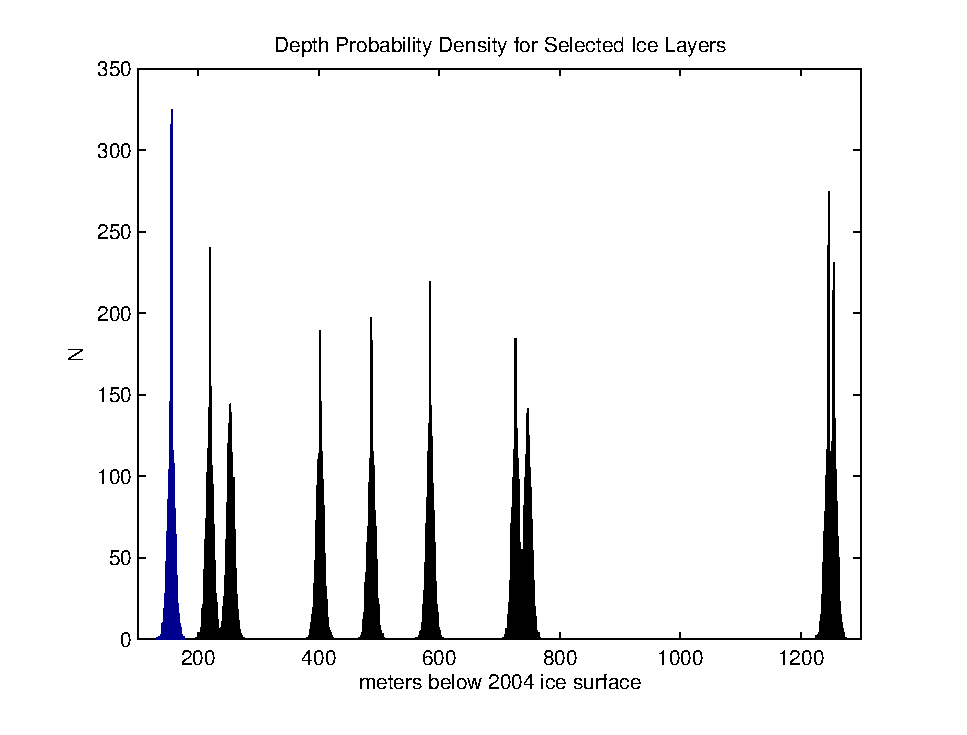
\includegraphics[scale=0.6]{depthhist_morland.eps}
	\label{depthhist}
	\caption{Histogram of modeled water-equivalent ice depth for each of 10 apparently prominent layers observed using airborne radar near Byrd Station, West Antarctica. The width of each distribution is the result of uncertainties arising from the method of radar collection, as discussed in Section~$\ref{method}$.}
\end{figure}

\begin{figure}
	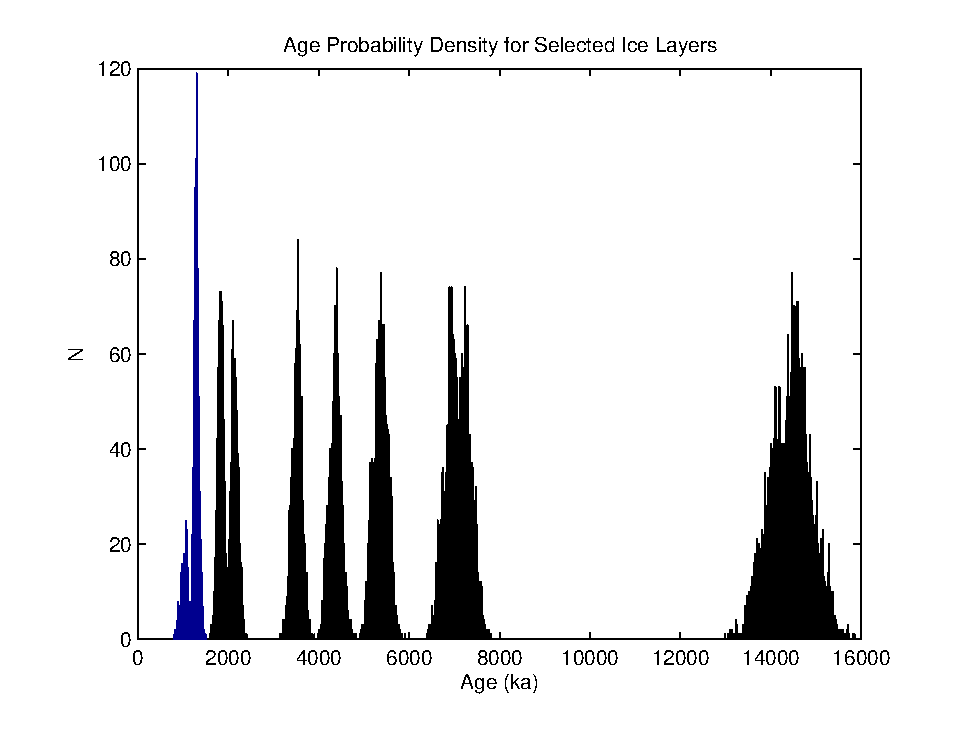
\includegraphics[scale=0.6]{agehist_morland.eps}
	\label{agehist}
	\caption{Histogram of the age distribution for each of 10 prominent layers observed using airborne radar near Byrd Station, West Antarctica. The distribution of ages associated with each layer represents the uncertainty in assigning ages to layers at varying depths. Age uncertainty stems from both radar uncertainty and isotopic ice core dating uncertainties.}
\end{figure}

\begin{figure}
	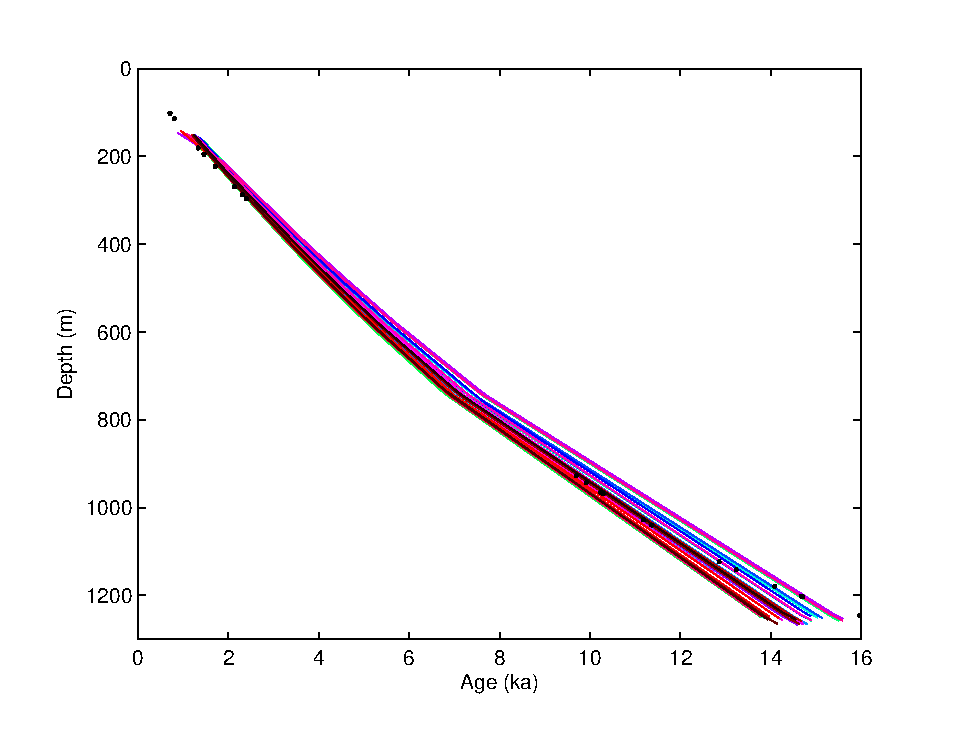
\includegraphics[scale=0.6]{spaghetti_morland.eps}
	\label{spaghetti}
	\caption{ Modeled age-depth distribution of layers observed using airborne radar near Byrd Station, West Antarctica. Black dots represent isotopically-dated volcanic events from the ice core record at Byrd Station. Each line represents a set of parameters (see Section~$\ref{method}$~that describe the observed data within uncertainty.    }
\end{figure}


%\begin{figure}
%	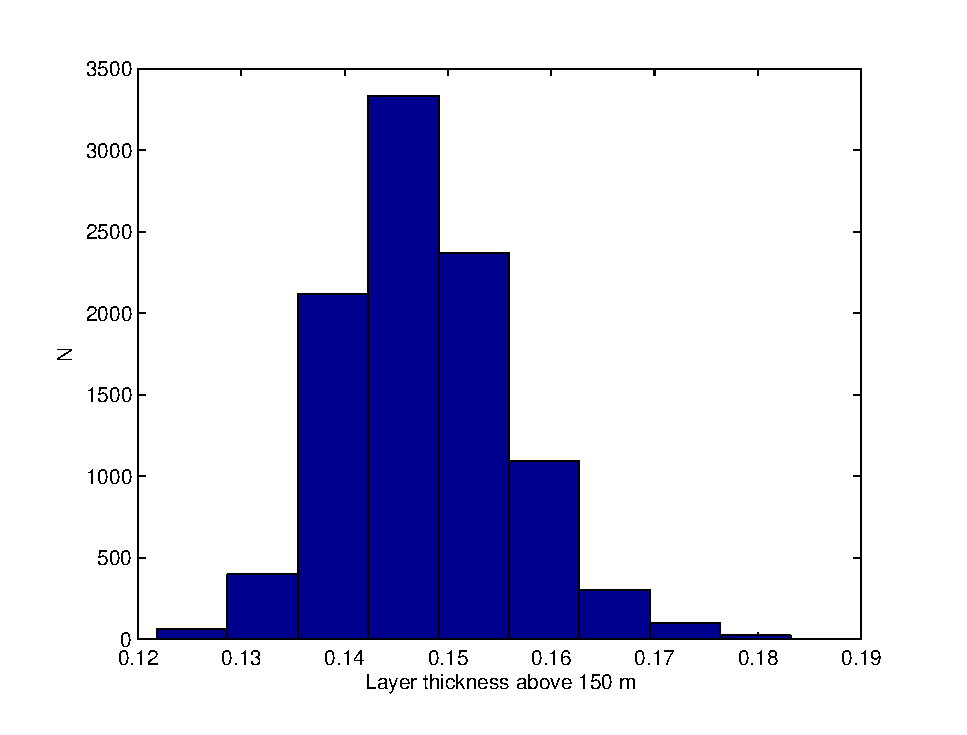
\includegraphics{thickgt150.eps}
%	\label{accum}
%	\caption{Modeled layer thickness in each of four depth regimes near Byrd Station, West Antarctica. **Check what observed is in each of these regimes to compare to mean of distribs** }
%\end{figure}
%\begin{figure}
%	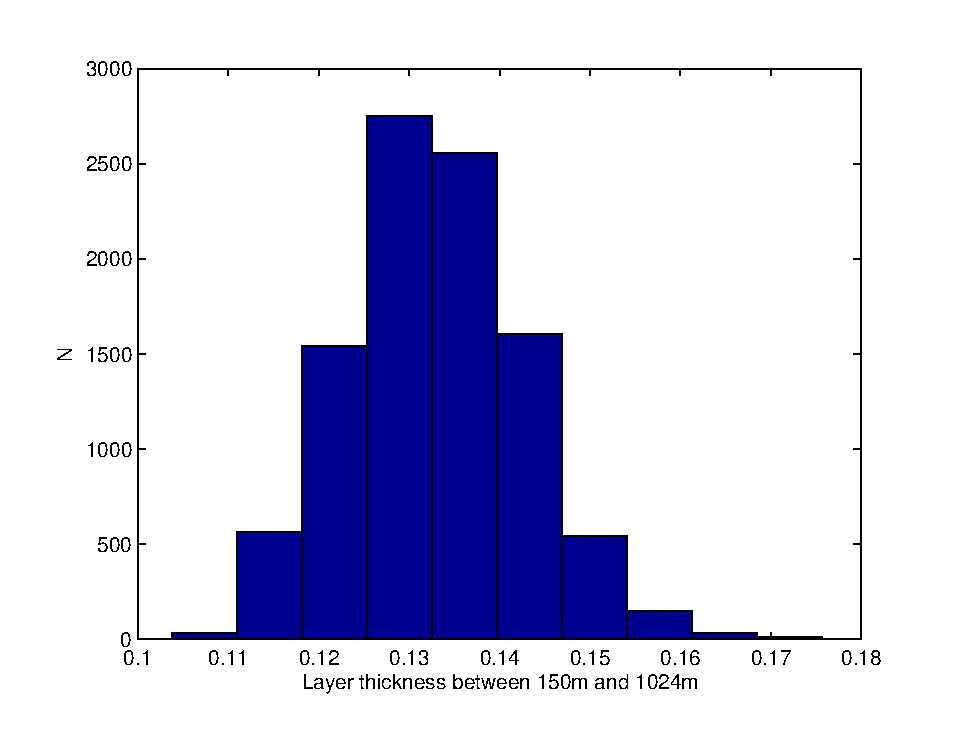
\includegraphics{thickgt1024lt150.eps}
%	\label{accum}
%	\caption{Modeled layer thickness in each of four depth regimes near Byrd Station, West Antarctica. **Check what observed is in each of these regimes to compare to mean of distribs** }
%\end{figure}
%\begin{figure}
%	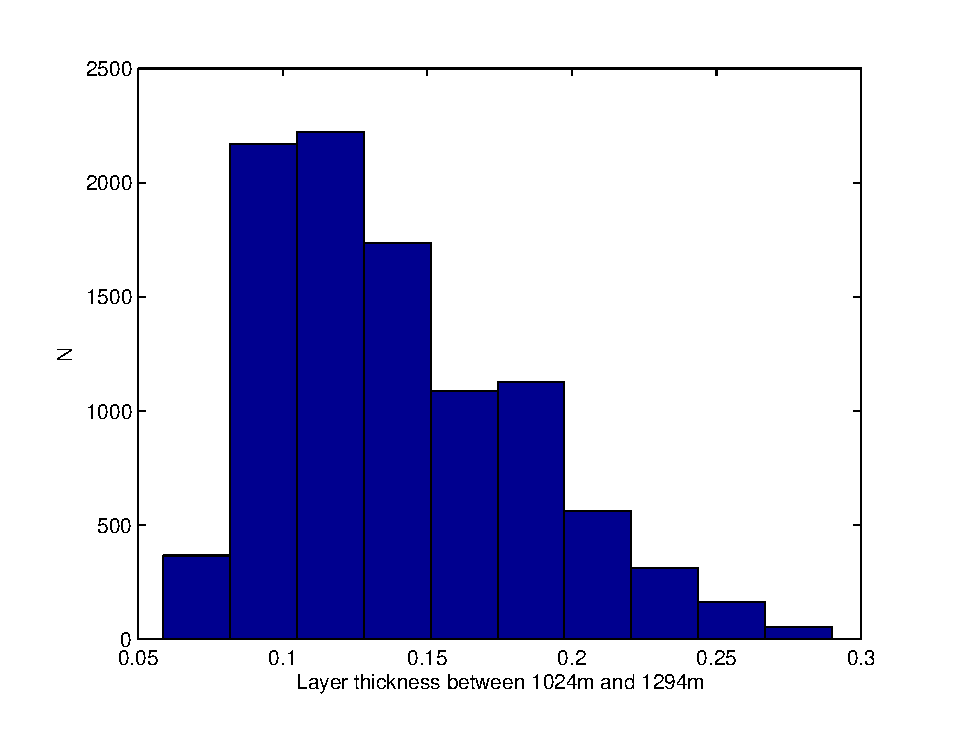
\includegraphics{thickgt1294lt150.eps}
%	\label{accum}
%	\caption{Modeled layer thickness in each of four depth regimes near Byrd Station, West Antarctica. **Check what observed is in each of these regimes to compare to mean of distribs** }
%\end{figure}
%\begin{figure}
%	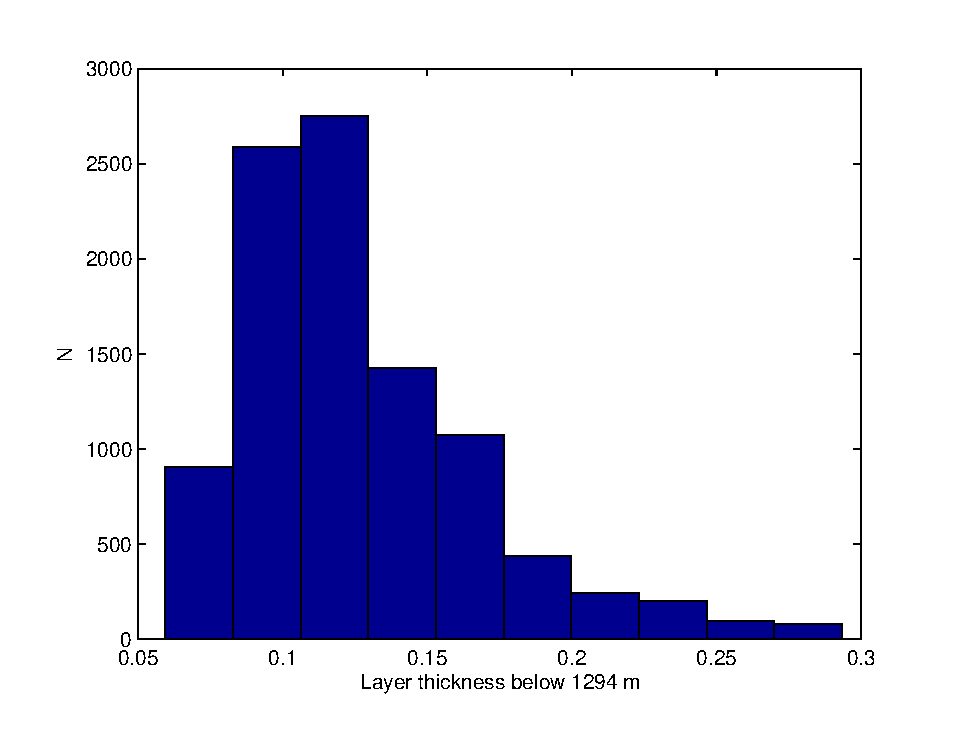
\includegraphics{thickgt1294.eps}
%	\label{accum}
%	\caption{Modeled layer thickness in each of four depth regimes near Byrd Station, West Antarctica. **Check what observed is in each of these regimes to compare to mean of distribs** }
%\end{figure}

\begin{figure}\label{accum}
\begin{center}$
\begin{array}{cc}
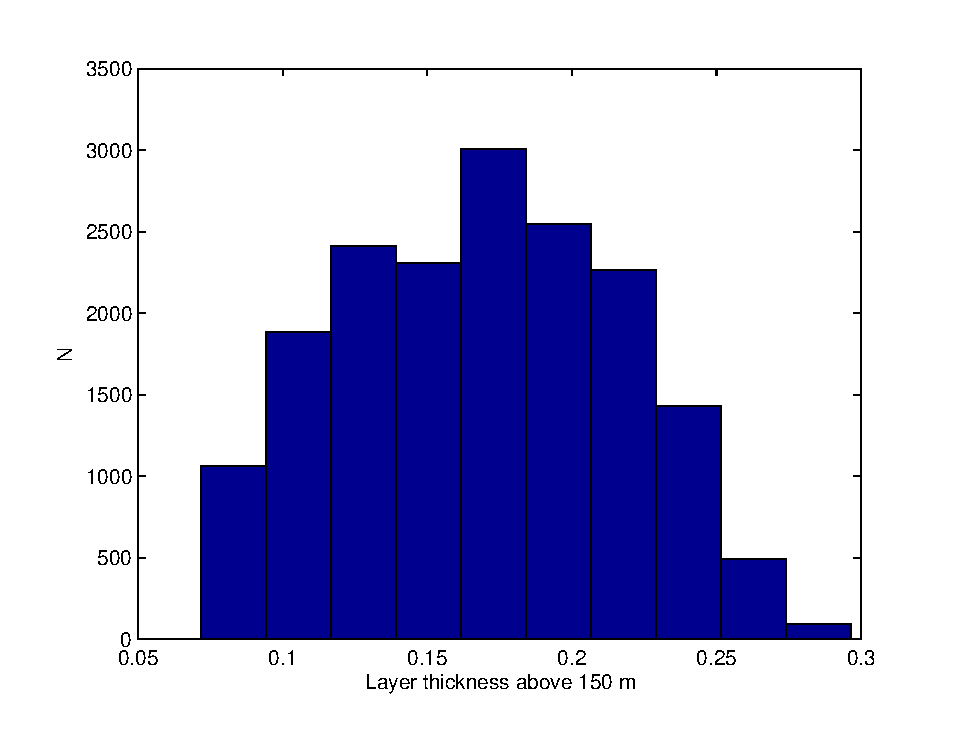
\includegraphics[width=2.5in]{thicklt150_morland.eps} &
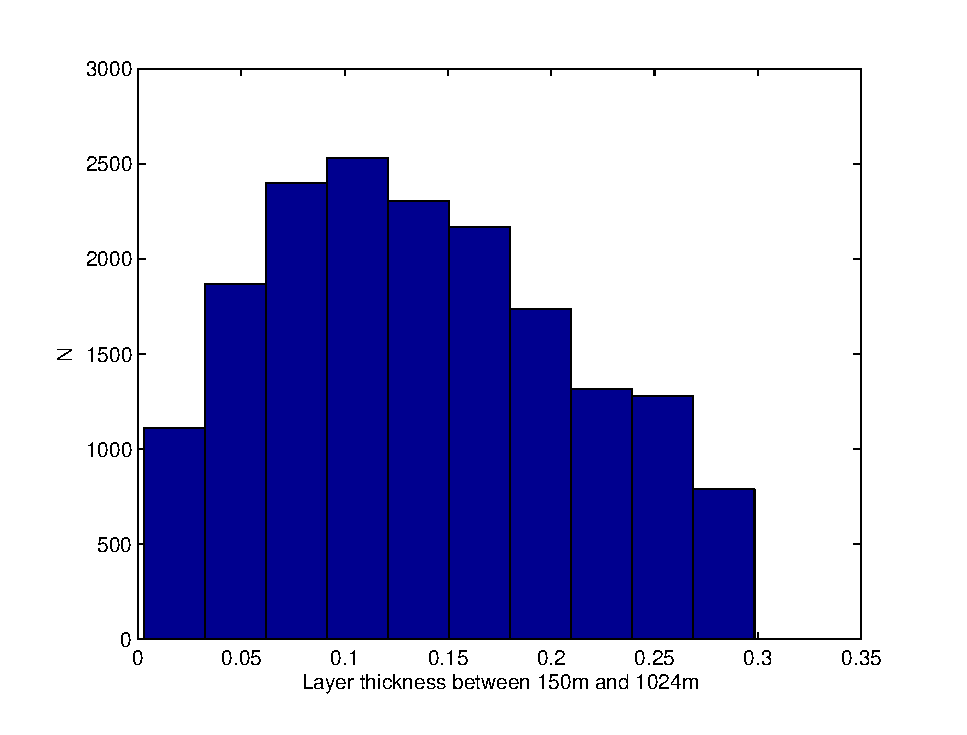
\includegraphics[width=2.5in]{thickgt150lt1024_morland.eps} \\ 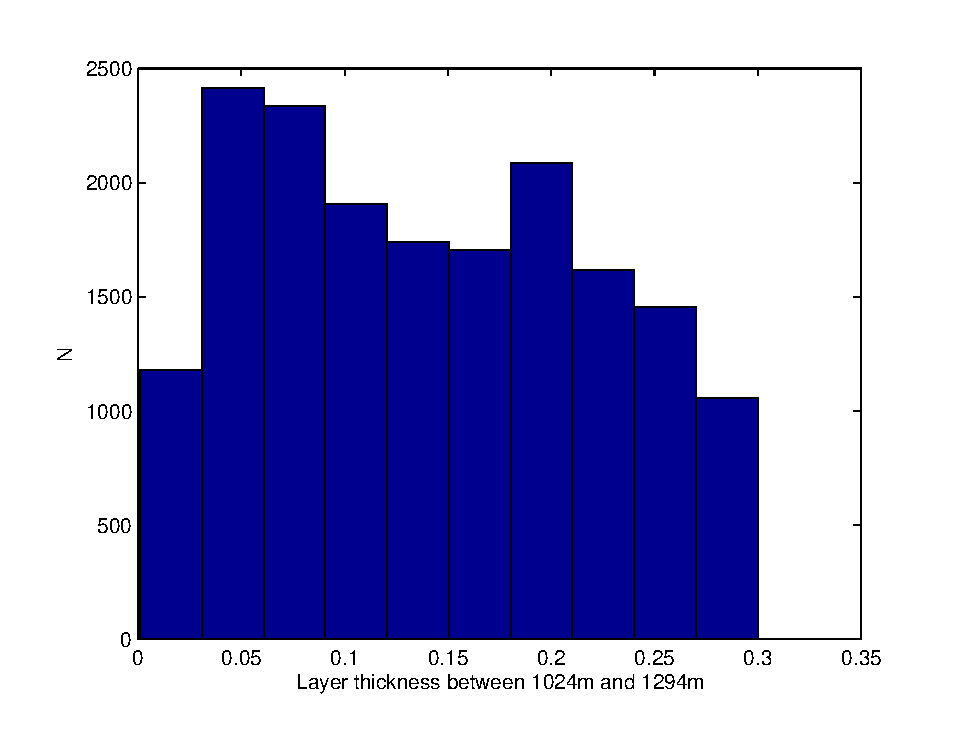
\includegraphics[width=2.5in]{thickgt1024lt1294_morland.eps} &
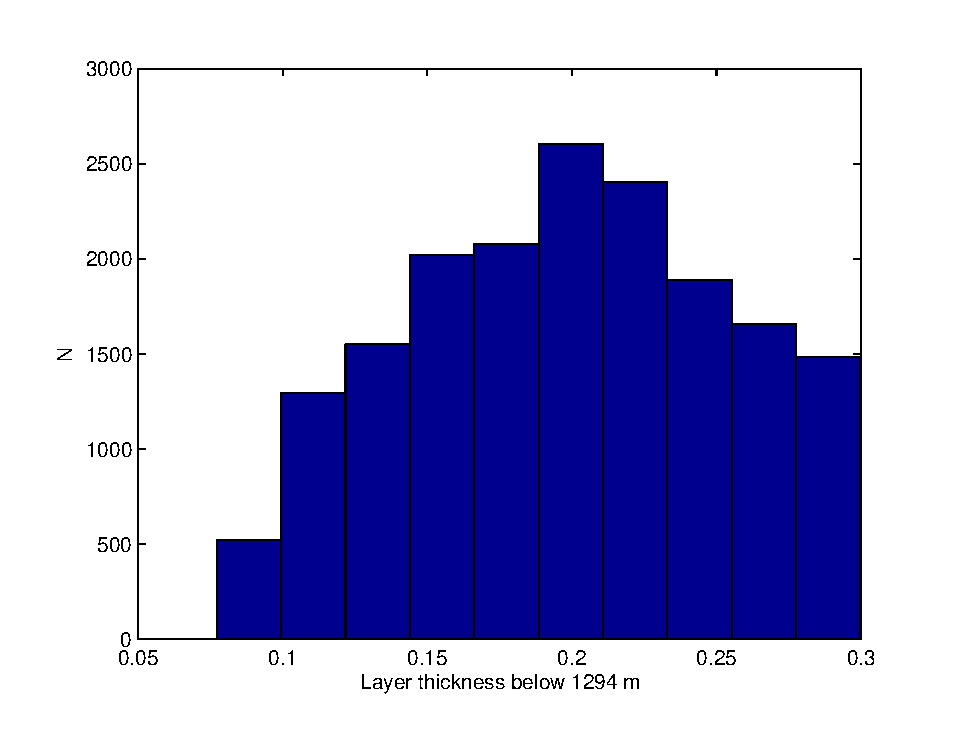
\includegraphics[width=2.5in]{thickgt1294_morland.eps}
\end{array}$
\end{center}
\caption{Modeled layer thickness in each of four depth regimes near Byrd Station, West Antarctica. The model overestimates layer thickness, particulary in deeper regimes. }
\end{figure}


\begin{table}\label{accums}
\caption{Comparison between layer thickness at the Western Divide between the Ross and Amundson Seas \citep{neumann2008} and modeled here at Byrd Station. Maximum layer thickness occurs at the divide, so layer thicknesses at Byrd Station are expected to be less, but comparable, at Byrd Station.}
\begin{tabular}{|c|c|c}
\hline
Depth Range (m) & Layer thickness at Divide (m/a) & Layer thickness at Byrd (m/a) \\
\hline
d $<$ 150 & $\sim$0.27 & $\sim$ 0.18 \\
150 $<$ d $<$ 1024 & $\sim$ 0.14 - 0.27 & $\sim$ 0.10\\
1024 $<$ d $<$ 1294 & $\sim$ 0.08 - 0.14 & $\sim$ 0.10\\
d $>$ 1294& $<$ 0.08 & $\sim$ 0.20\\
\hline
\end{tabular}
\end{table}

\begin{table}\label{age_unc}
\caption{Uncertainty in ice core dates based on analysis by \citet{schwander2001} for Dome C, Antarctica. Age uncertainty is considered to be gaussian with standard deviation from a variety of age reference points.}
\begin{tabular}{|p{4cm}|p{4cm}|p{8cm}|}
\hline
 Age (a) & 1$\sigma$ Uncertainty (a) & Method of Dating  \\
\hline
&&\\
Age $<$ 1360 & $\pm$ 10  & volcanic events (historically documented or fit to Vostok GT4 scale \citep{Petit1999}\\
& & \\
1360 $\ge$ Age $>$ 11500 & $\pm$ 100  & end of Younger Dryas period and $^{10}Be$ peak \\
&& \\
11500 $\ge$ Age $>$ 17320 & $\pm$ 510 & significant volcanic event "Old Faithful" from \citet{hammer1994}\\
&&\\
Age $\ge$ 17320 & $\pm$ 2000 & U/Th dating of Laschamp geomagnatic excursion \citep{schramm2000}\\
\hline
\end{tabular}
%\tablenotetext{a}{Footnote text here.}
\end{table}



\begin{table}\label{results}
\caption{Depth and age mean, median, and uncertainty for 10 strong radar reflectors near Byrd Station, West Antarctica. The radar two-way travel time (TWTT) is given in column 1. }
\centering
\begin{tabular}{| l || l | l | c || c | c | c |}
\hline
\multirow{2}{*}{TWTT (us)} &  \multicolumn{3}{c||}{Depth (m)} & \multicolumn{3}{c|}{Age (a)} \\   
\cline{2-7}
 & Mean & Median & Std Dev & Mean & Median & Std Dev \\
\hline
 6.02   & 155.5  & 155.2  & 5.5953 & 1246. & 1277. & 119   \\
 6.775  & 219.4  & 219.7  & 5.6589 & 1832. & 1831. & 73   \\
 7.18   & 253.6  & 254.0  & 5.6603 & 2136. & 2136. & 80  \\
 8.94   & 402.4  & 402.5  & 5.6783 & 3516. & 3517. & 115   \\
 9.9402 & 487.6  & 487.5  & 5.6148 & 4358. & 4361. & 138   \\
 11.1   & 584.9  & 584.7  & 5.6491 & 5370. & 5374. & 166   \\
 12.78  & 726.8  & 726.8  & 5.5936 & 6957. & 6964. & 211   \\
 13.02  & 747.1  & 746.9  & 5.6039 & 7196. & 7202. & 216   \\
 18.92  & 1245.8 & 1246.3 & 5.7603 & 14,352. & 14,370. & 428   \\
 19.0205 & 1254.2 & 1254.6 & 5.6922 & 14,503. & 14,518. & 434  \\
\hline
\end{tabular}
%\tablenotetext{a}{Footnote text here.}
\end{table}

\end{document}
